\title{Midterm 2}
\author{Dr. Jordan Hanson - Whittier College Dept. of Physics and Astronomy}
\date{\today}
\documentclass[10pt]{article}
\usepackage[a4paper, total={18cm, 27cm}]{geometry}
\usepackage{outlines}
\usepackage{graphicx}
\begin{document}
\maketitle

\section{Chapter 5 - Combinatorial Logic Analysis}
\label{sec:comb}

\begin{enumerate}
\item Imagine we have a keypad that has digits 0-9 and and letters A-F.  Assume each key sends an active-LOW signal to an encoder that converts the single key value to binary.  For example, if one presses $A$, the 4-bit output is 1010.  Write the conversion table for the digits and letters to binary below, and develop the encoder logic that produces the binary outputs. \\
\begin{table}[ht]
\centering
\begin{tabular}{| c | c | c |}
\hline
\hline
Input & Encoded to Binary & Logic Expression \\
0 & 0000 (Omit) & None, no connect \\ 
1 & 0001 & $d_0 d_1 d_2 \bar{d}_3$ \\ 
2 & 0010 & $d_0 d_1 \bar{d}_2 d_3$ \\ 
3 & 0011 & $d_0 d_1 \bar{d}_2 \bar{d}_3$ \\ 
4 & 0100 & $d_0 \bar{d}_1 d_2 d_3$ \\
5 & 0101 & $d_0 \bar{d}_1 d_2 \bar{d}_3$ \\ 
6 & 0110 & $d_0 \bar{d}_1 \bar{d}_2 d_3$ \\ 
7 & 0111 & $d_0 \bar{d}_1 \bar{d}_2 \bar{d}_3$ \\ 
8 & 1000 & $\bar{d}_0 d_1 d_2 d_3$ \\ 
9 & 1001 & $\bar{d}_0 d_1 d_2 \bar{d}_3$ \\ 
A & 1010 & $\bar{d}_0 d_1 \bar{d}_2 d_3$ \\ 
B & 1011 & $\bar{d}_0 d_1 \bar{d}_2 \bar{d}_3$ \\ 
C & 1100 & $\bar{d}_0 \bar{d}_1 d_2 d_3$ \\ 
D & 1101 & $\bar{d}_0 \bar{d}_1 d_2 \bar{d}_3$ \\ 
E & 1110 & $\bar{d}_0 \bar{d}_1 \bar{d}_2 d_3$ \\ 
F & 1111 & $\bar{d}_0 \bar{d}_1 \bar{d}_2 \bar{d}_3$ \\ \hline
\hline
\end{tabular} \hspace{0.5cm}
\caption{\label{tab:tab1} Solution to Ch. 5 ex. 1. A table for the hexadecimal encodings.}
\end{table}
\begin{figure}[hb]
\centering
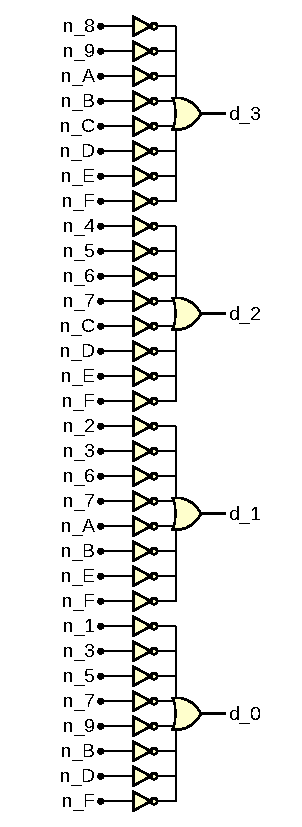
\includegraphics[width=0.18\textwidth,trim=0cm 0cm 0cm 0cm,clip=true]{figures/gateExample9.pdf}
\caption{\label{fig:encoder} Solution to Ch. 5 ex 1.  The circuit diagram for the hex encoder.}
\end{figure}

\item The output waveform in Fig. \ref{fig:gates1} is incorrect for the inputs that are applied to the circuit.  Assuming that one gate in the circuit has failed, with its output either an apparent constant HIGH or a constant LOW, determine the faulty gate and the type of failure (output open or shorted). \\ \\
In the third time step, we see ABC = 111, which should lead to a HIGH on the output.  The fault cannot be with G4 because X is HIGH appropriately when D = 1 and E = 0.  This also implies that G3 is OK.  In the middle times step, ABC = 100 and we see X = 0, which is right, but that doesn't reveal if G1 or G2 is stuck LOW.  Answer: G1 or G2 is stuck LOW.
\end{enumerate}

\begin{figure}[ht]
\centering
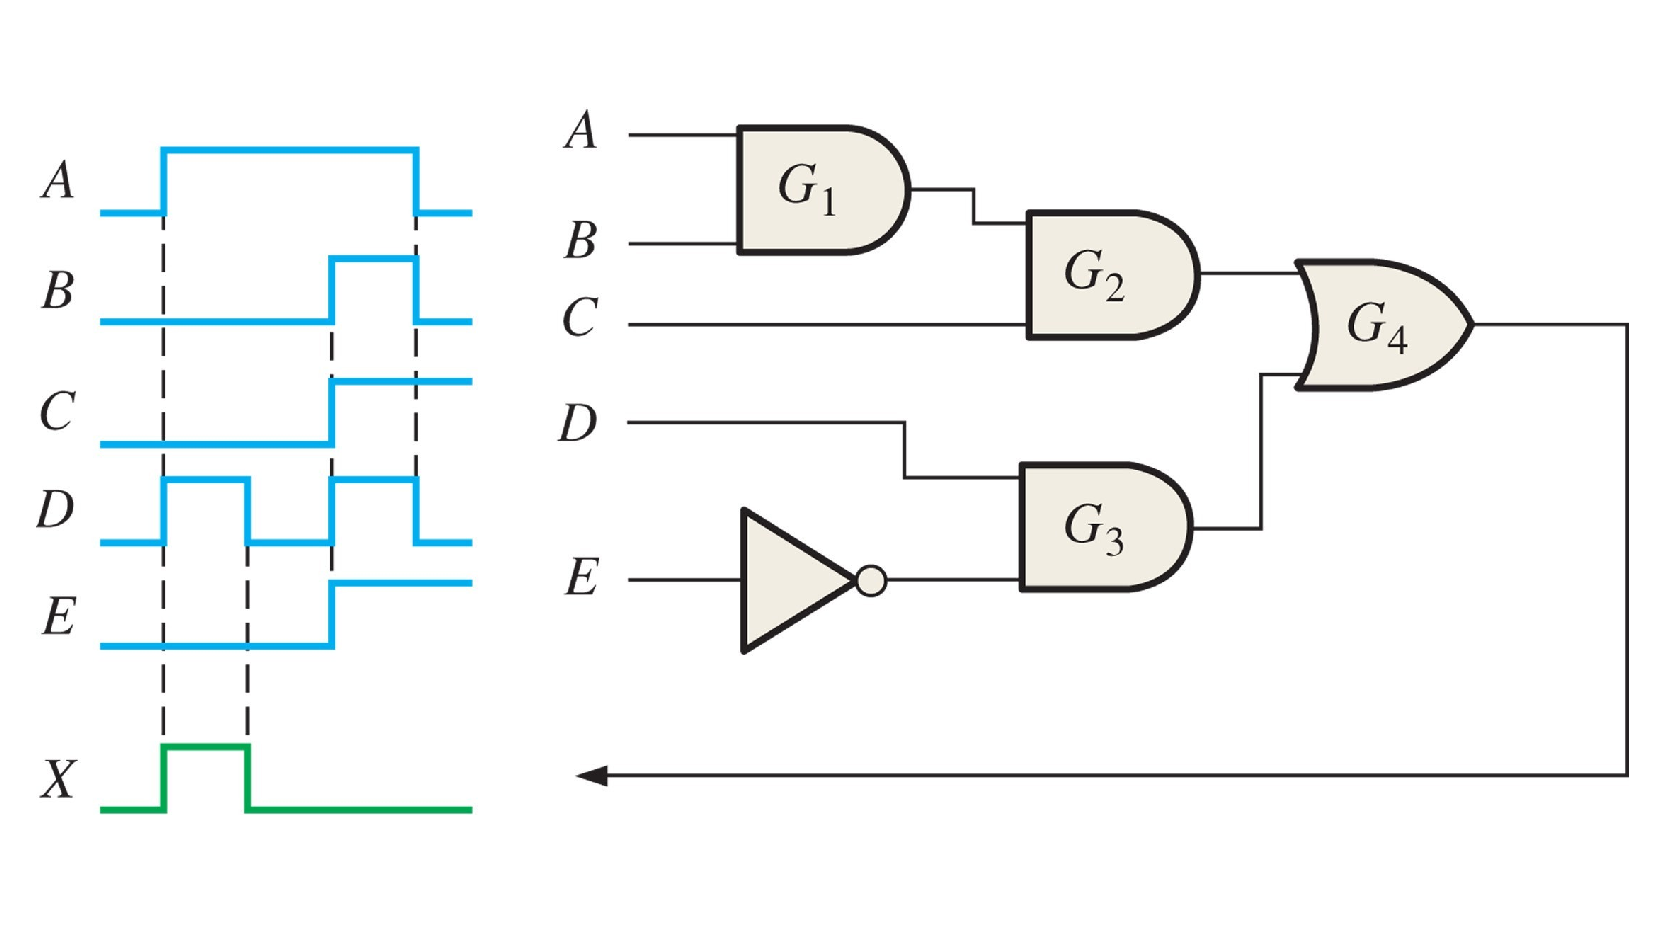
\includegraphics[width=0.4\textwidth]{figures/troubleshoot.pdf}
\caption{\label{fig:gates1} A domain-5 logic function needs debugging.}
\end{figure}

\section{Chapter 6 - Functions of Combinational Logic}
\label{sec:comb2}

\begin{figure}[ht]
\centering
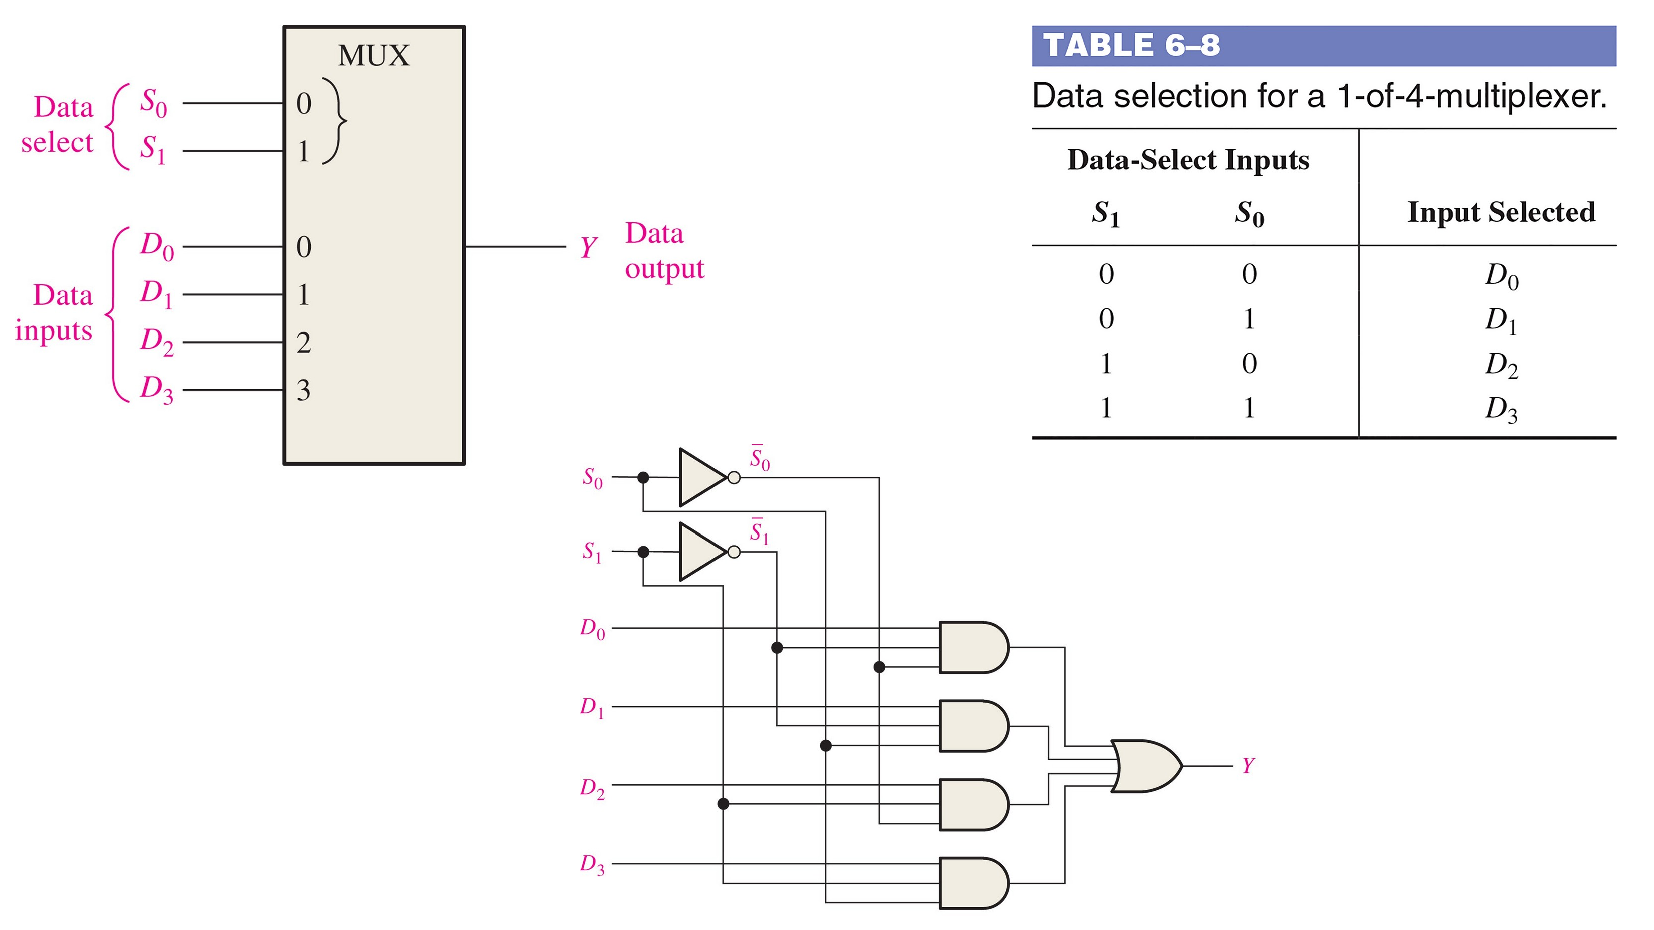
\includegraphics[width=0.5\textwidth]{figures/mux4.pdf}
\caption{\label{fig:mux4} A 1-of-4 multiplexer (mux) logic function: function block, truth table, and gate diagram.}
\end{figure}

\begin{enumerate}
\item Consider Fig. \ref{fig:mux4}, in which the 1-of-4 mux is reviewed.  Imagine a camera system (like Zoom only with firmware) in which you are switching between four data feeds from four cameras by holding down one of four different keys.  Design a circuit using an encoder and a 1-of-4 mux to switch between four bitstreams on active-LOW keypresses from four keys. Show the encoder logic at the gate level. \\ \\
\begin{table}[hb]
\centering
\begin{tabular}{| c | c | c |}
\hline
\hline
Key pressed & Binary code & Active-LOW outputs \\
A & 00 & Not connected \\
B & 01 & $d_0 \bar{d}_1$ \\
C & 10 & $\bar{d}_0 d_1$ \\
D & 11 & $\bar{d}_0 \bar{d}_1$ \\
\hline
\hline
\end{tabular}
\caption{\label{tab:mux} Solution to Ch. 6 ex. 1.  A table demonstrating the states of the active-LOW encoder.}
\end{table}
\begin{figure}
\centering
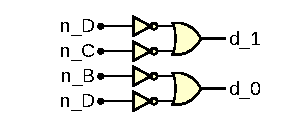
\includegraphics[width=0.35\textwidth]{figures/gateExample10.pdf}
\caption{\label{fig:muxDecode} Solution to Ch. 6 ex. 1.  The encoder portion.}
\end{figure}
Consider the entries in Tab. \ref{tab:mux} and the circuit in Fig. \ref{fig:muxDecode}.  The 1-of-4 mux is controlled by the encoder, which follows the data in the table.  The bitstreams A-D are the inputs to the mux. \\ \\
\item Using XNOR gates, we could create a comparator that is true if two 2-bit binary numbers are equal.  Starting with the 2-bit comparator, add logic that is true if $A>B$.  Add one final output that is the opposite of $A>B$ (so $A<B$)\footnote{Since this is a 2-bit system, you can enumerate all possible states, if that helps.}. \\ \\ 
A 2-bit comparator with greater-than and less-than outputs is depicted in Fig. \ref{fig:comp}.  The $A=B$ portion is composed of two XNOR gates and an AND gate.  The $A > B$ output is composed of three AND gates and an OR gate.  The $A < B$ output is HIGH if the other two outputs are LOW.
\begin{figure}
\centering
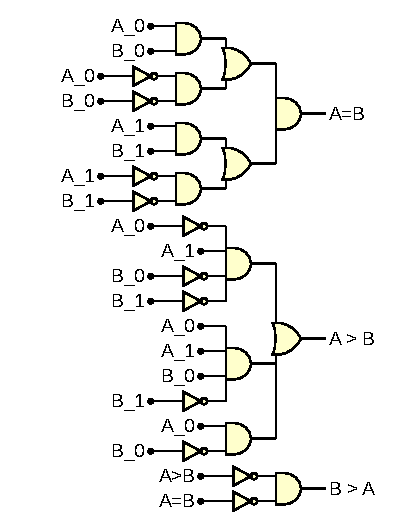
\includegraphics[width=0.3\textwidth]{figures/gateExample11.pdf}
\caption{\label{fig:comp} Solution to Ch. 6 ex. 2.}
\end{figure}
\end{enumerate}

\section{Chapter 7 - Latches, Flip-flops, and Timers}
\label{sec:latch}

\begin{figure}[ht]
\centering
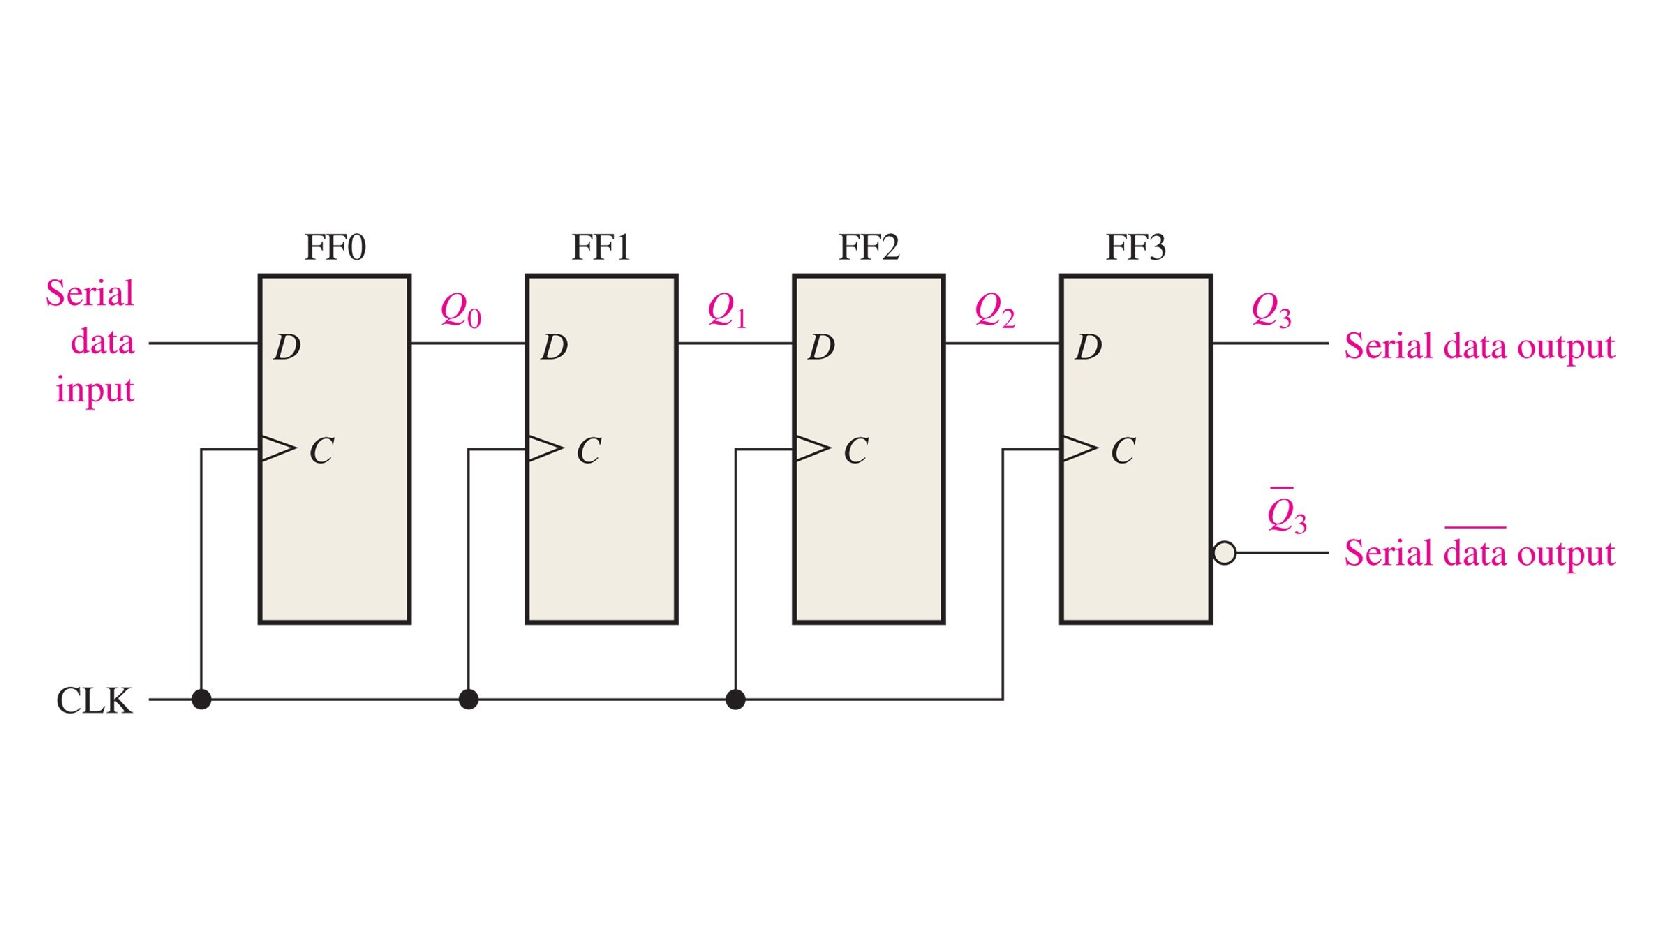
\includegraphics[width=0.5\textwidth,trim=0cm 2cm 0cm 2cm,clip=true]{figures/latches2.pdf}
\caption{\label{fig:latches} This is an example of a serial-in serial-out shift register.}
\end{figure}

\begin{enumerate}
\item Consider Fig. \ref{fig:latches}, in which four D flip-flops are connected in series to form a \textit{shift register.}  (a) Produce the timing diagram that occurs on the serial data output when all four D flip-flops are initially in the RESET state, and a single data bit arrives at the input with a constantly-running clock signal.  (b) Add an input that disables the clock to halt the shift register so that the data is stored.  Draw a timing diagram showing the shifting of 4 bits into the register and halting on the right clock cycle to store them. \\ 
\begin{figure}[ht]
\centering
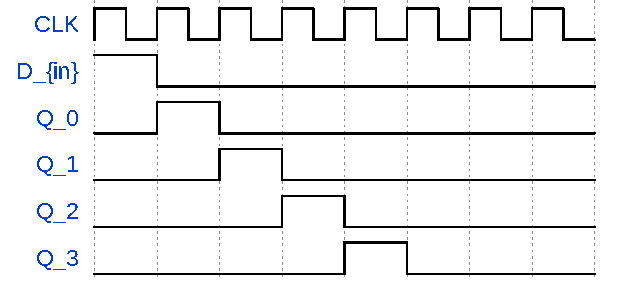
\includegraphics[width=0.4\textwidth]{figures/timingExample12.pdf} \hspace{0.5cm}
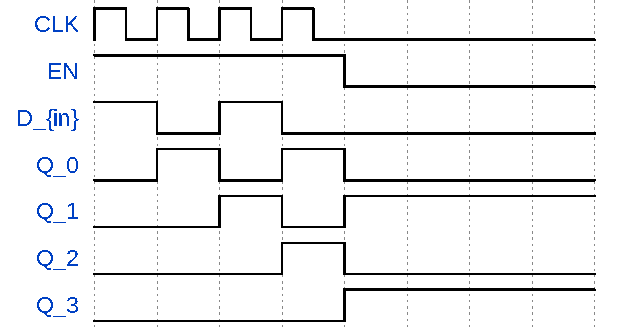
\includegraphics[width=0.4\textwidth]{figures/timingExample13.pdf}
\caption{\label{fig:shift} Solution to Ch. 7 ex. 1. (Left) Operating the shift register for 8 clock cycles. (Right) Passing 4 bits into the shift register and halting the clock to keep the D flip-flops stable.}
\end{figure}

Figure \ref{fig:shift} shows the timing diagrams required by parts (a) and (b).  Subsquent D flip-flops follow prior flip-flops, if the clock moves them on positive edges. When the enable signal goes LOW, the clock stops and the flip-flops retain their states. \\
\item Create a function block to represent the 4-bit shift register from the previous problem.  Now design a system that adds two binary numbers and stores the result in the shift register via a 1-of-4 multiplexer.  The mux is there to convert the \textit{parallel} data out of the adder to \textit{serial} data into the register. (Continue response on back). \\ 
\begin{figure}
\centering
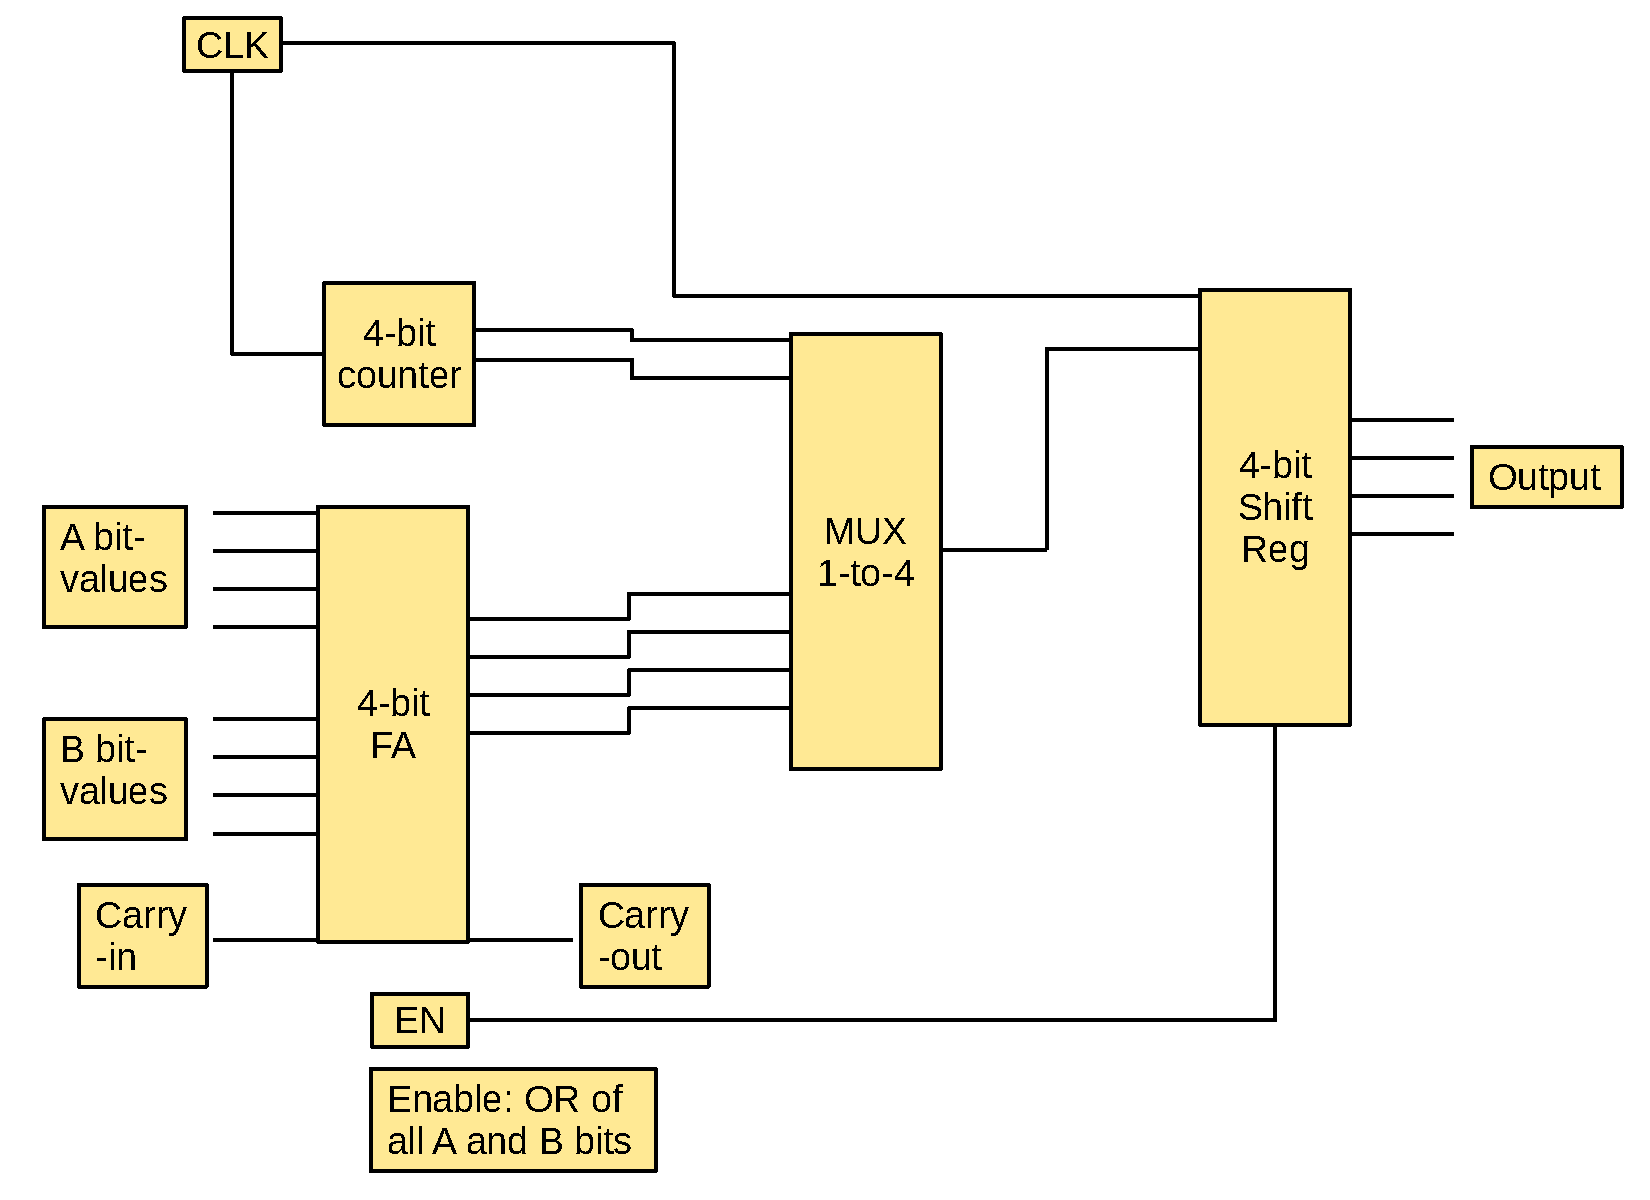
\includegraphics[width=0.65\textwidth]{figures/design4.pdf}
\caption{\label{fig:addMux} Design for Ch. 7 ex. 2.}
\end{figure}
In Fig. \ref{fig:addMux}.  The binary values of the numbers A and B, plus carry-in, enter the full adder at left.  The result of the adder feeds into the multiplexer.  The clock runs a 2-bit counter that runs from 0-3 repeatedly.  The counter runs the data select lines of the multiplexer.  The LSB to MSB are passed in order, serially, to the shift-register.  The register is enabled only when there are numbers present in the adder, and moves on the clock signal.  It is assumed that the adder inputs are held constant until the register captures the results.
\end{enumerate}

\end{document}